\chapter{Mengenal Kecerdasan Buatan dan Scikit-Learn}
Buku umum yang digunakan adalah \cite{russell2016artificial} dan
untuk sebelum UTS menggunakan buku \textit{Python Artificial Intelligence Projects for Beginners}\cite{eckroth2018python}.
Dengan praktek menggunakan python 3 dan editor anaconda dan library python scikit-learn.
Tujuan pembelajaran pada pertemuan pertama antara lain:
\begin{enumerate}
\item
Mengerti definisi kecerdasan buatan, sejarah kecerdasan buatan, perkembangan dan penggunaan di perusahaan
\item
Memahami cara instalasi dan pemakaian sci-kit learn
\item
Memahami cara penggunaan variabel explorer di spyder
\end{enumerate}
Tugas dengan cara dikumpulkan dengan pull request ke github dengan menggunakan latex pada repo yang dibuat oleh asisten riset.

\section{Teori}
Praktek teori penunjang yang dikerjakan :
\begin{enumerate}
\item
Buat Resume Definisi, Sejarah dan perkembangan Kecerdasan Buatan, dengan bahasa yang mudah dipahami dan dimengerti. Buatan sendiri bebas plagiat[hari ke 1](10)
\item
Buat Resume mengenai definisi supervised learning, klasifikasi, regresi dan unsupervised learning. Data set, training set dan testing set.[hari ke 1](10)
\end{enumerate}

\section{Instalasi}
Membuka https://scikit-learn.org/stable/tutorial/basic/tutorial.html. Dengan menggunakan bahasa yang mudah dimengerti dan bebas plagiat.
Dan wajib skrinsut dari komputer sendiri.
\begin{enumerate}
\item
Instalasi library scikit dari anaconda, mencoba kompilasi dan uji coba ambil contoh kode dan lihat variabel explorer[hari ke 1](10)
\item
Mencoba Loading an example dataset, menjelaskan maksud dari tulisan tersebut dan mengartikan per baris[hari ke 1](10)
\item
Mencoba Learning and predicting, menjelaskan maksud dari tulisan tersebut dan mengartikan per baris[hari ke 2](10)
\item
mencoba Model persistence, menjelaskan maksud dari tulisan tersebut dan mengartikan per baris[hari ke 2](10)
\item
Mencoba Conventions, menjelaskan maksud dari tulisan tersebut dan mengartikan per baris[hari ke 2](10)
\end{enumerate}


\section{Penanganan Error}
Dari percobaan yang dilakukan di atas, apabila mendapatkan error maka:

\begin{enumerate}
	\item
	skrinsut error[hari ke 2](10)
	\item
Tuliskan kode eror dan jenis errornya [hari ke 2](10)
	\item
Solusi pemecahan masalah error tersebut[hari ke 2](10)

\end{enumerate}

\chapter{Mengenal Kecerdasan Buatan dan Scikit-Learn}
Buku umum yang digunakan adalah \cite{russell2016artificial} dan
untuk sebelum UTS menggunakan buku \textit{Python Artificial Intelligence Projects for Beginners}\cite{eckroth2018python}.
Dengan praktek menggunakan python 3 dan editor anaconda dan library python scikit-learn.
Tujuan pembelajaran pada pertemuan pertama antara lain:
\begin{enumerate}
\item
Mengerti definisi kecerdasan buatan, sejarah kecerdasan buatan, perkembangan dan penggunaan di perusahaan
\item
Memahami cara instalasi dan pemakaian sci-kit learn
\item
Memahami cara penggunaan variabel explorer di spyder
\end{enumerate}
Tugas dengan cara dikumpulkan dengan pull request ke github dengan menggunakan latex pada repo yang dibuat oleh asisten riset.

\section{Teori}
Praktek teori penunjang yang dikerjakan :
\begin{enumerate}
\item
Buat Resume Definisi, Sejarah dan perkembangan Kecerdasan Buatan, dengan bahasa yang mudah dipahami dan dimengerti. Buatan sendiri bebas plagiat[hari ke 1](10)
\item
Buat Resume mengenai definisi supervised learning, klasifikasi, regresi dan unsupervised learning. Data set, training set dan testing set.[hari ke 1](10)
\end{enumerate}

\section{Instalasi}
Membuka https://scikit-learn.org/stable/tutorial/basic/tutorial.html. Dengan menggunakan bahasa yang mudah dimengerti dan bebas plagiat.
Dan wajib skrinsut dari komputer sendiri.
\begin{enumerate}
\item
Instalasi library scikit dari anaconda, mencoba kompilasi dan uji coba ambil contoh kode dan lihat variabel explorer[hari ke 1](10)
\item
Mencoba Loading an example dataset, menjelaskan maksud dari tulisan tersebut dan mengartikan per baris[hari ke 1](10)
\item
Mencoba Learning and predicting, menjelaskan maksud dari tulisan tersebut dan mengartikan per baris[hari ke 2](10)
\item
mencoba Model persistence, menjelaskan maksud dari tulisan tersebut dan mengartikan per baris[hari ke 2](10)
\item
Mencoba Conventions, menjelaskan maksud dari tulisan tersebut dan mengartikan per baris[hari ke 2](10)
\end{enumerate}


\section{Penanganan Error}
Dari percobaan yang dilakukan di atas, apabila mendapatkan error maka:

\begin{enumerate}
	\item
	skrinsut error[hari ke 2](10)
	\item
Tuliskan kode eror dan jenis errornya [hari ke 2](10)
	\item
Solusi pemecahan masalah error tersebut[hari ke 2](10)

\end{enumerate}

\chapter{Mengenal Kecerdasan Buatan dan Scikit-Learn}
Buku umum yang digunakan adalah \cite{russell2016artificial} dan
untuk sebelum UTS menggunakan buku \textit{Python Artificial Intelligence Projects for Beginners}\cite{eckroth2018python}.
Dengan praktek menggunakan python 3 dan editor anaconda dan library python scikit-learn.
Tujuan pembelajaran pada pertemuan pertama antara lain:
\begin{enumerate}
\item
Mengerti definisi kecerdasan buatan, sejarah kecerdasan buatan, perkembangan dan penggunaan di perusahaan
\item
Memahami cara instalasi dan pemakaian sci-kit learn
\item
Memahami cara penggunaan variabel explorer di spyder
\end{enumerate}
Tugas dengan cara dikumpulkan dengan pull request ke github dengan menggunakan latex pada repo yang dibuat oleh asisten riset.

\section{Teori}
Praktek teori penunjang yang dikerjakan :
\begin{enumerate}
\item
Buat Resume Definisi, Sejarah dan perkembangan Kecerdasan Buatan, dengan bahasa yang mudah dipahami dan dimengerti. Buatan sendiri bebas plagiat[hari ke 1](10)
\item
Buat Resume mengenai definisi supervised learning, klasifikasi, regresi dan unsupervised learning. Data set, training set dan testing set.[hari ke 1](10)
\end{enumerate}

\section{Instalasi}
Membuka https://scikit-learn.org/stable/tutorial/basic/tutorial.html. Dengan menggunakan bahasa yang mudah dimengerti dan bebas plagiat.
Dan wajib skrinsut dari komputer sendiri.
\begin{enumerate}
\item
Instalasi library scikit dari anaconda, mencoba kompilasi dan uji coba ambil contoh kode dan lihat variabel explorer[hari ke 1](10)
\item
Mencoba Loading an example dataset, menjelaskan maksud dari tulisan tersebut dan mengartikan per baris[hari ke 1](10)
\item
Mencoba Learning and predicting, menjelaskan maksud dari tulisan tersebut dan mengartikan per baris[hari ke 2](10)
\item
mencoba Model persistence, menjelaskan maksud dari tulisan tersebut dan mengartikan per baris[hari ke 2](10)
\item
Mencoba Conventions, menjelaskan maksud dari tulisan tersebut dan mengartikan per baris[hari ke 2](10)
\end{enumerate}


\section{Penanganan Error}
Dari percobaan yang dilakukan di atas, apabila mendapatkan error maka:

\begin{enumerate}
	\item
	skrinsut error[hari ke 2](10)
	\item
Tuliskan kode eror dan jenis errornya [hari ke 2](10)
	\item
Solusi pemecahan masalah error tersebut[hari ke 2](10)

\end{enumerate}

\chapter{Mengenal Kecerdasan Buatan dan Scikit-Learn}
Buku umum yang digunakan adalah \cite{russell2016artificial} dan
untuk sebelum UTS menggunakan buku \textit{Python Artificial Intelligence Projects for Beginners}\cite{eckroth2018python}.
Dengan praktek menggunakan python 3 dan editor anaconda dan library python scikit-learn.
Tujuan pembelajaran pada pertemuan pertama antara lain:
\begin{enumerate}
\item
Mengerti definisi kecerdasan buatan, sejarah kecerdasan buatan, perkembangan dan penggunaan di perusahaan
\item
Memahami cara instalasi dan pemakaian sci-kit learn
\item
Memahami cara penggunaan variabel explorer di spyder
\end{enumerate}
Tugas dengan cara dikumpulkan dengan pull request ke github dengan menggunakan latex pada repo yang dibuat oleh asisten riset.
\endchapter

\section{Teori}
Praktek teori penunjang yang dikerjakan :
\begin{enumerate}
\item
Buat Resume Definisi, Sejarah dan perkembangan Kecerdasan Buatan, dengan bahasa yang mudah dipahami dan dimengerti. Buatan sendiri bebas plagiat[hari ke 1](10)
\item
Buat Resume mengenai definisi supervised learning, klasifikasi, regresi dan unsupervised learning. Data set, training set dan testing set.[hari ke 1](10)
\end{enumerate}

\section{Instalasi}
Membuka https://scikit-learn.org/stable/tutorial/basic/tutorial.html. Dengan menggunakan bahasa yang mudah dimengerti dan bebas plagiat.
Dan wajib skrinsut dari komputer sendiri.
\begin{enumerate}
\item
Instalasi library scikit dari anaconda, mencoba kompilasi dan uji coba ambil contoh kode dan lihat variabel explorer[hari ke 1](10)
\item
Mencoba Loading an example dataset, menjelaskan maksud dari tulisan tersebut dan mengartikan per baris[hari ke 1](10)
\item
Mencoba Learning and predicting, menjelaskan maksud dari tulisan tersebut dan mengartikan per baris[hari ke 2](10)
\item
mencoba Model persistence, menjelaskan maksud dari tulisan tersebut dan mengartikan per baris[hari ke 2](10)
\item
Mencoba Conventions, menjelaskan maksud dari tulisan tersebut dan mengartikan per baris[hari ke 2](10)
\end{enumerate}


\section{Penanganan Error}
Dari percobaan yang dilakukan di atas, apabila mendapatkan error maka:

\begin{enumerate}
	\item
	skrinsut error[hari ke 2](10)
	\item
Tuliskan kode eror dan jenis errornya [hari ke 2](10)
	\item
Solusi pemecahan masalah error tersebut[hari ke 2](10)

\end{enumerate}

\section{Teori}
Teori mencakup resume dari beberapa pembahasan. yaitu :
\begin{enumerate}
\item Definisi Kecerdasan Buatan.

Kecerdasan buatan (Artificial Intelligence) atau disingkat menjadi AI adalah suatu pengetahuan yang membuat suatu komputer dapat menirkan  kecerdasan manusia sehingga diharapkan atau diinginkan komputer dapat melakukan hal-hal yang apabila dikerjakan manusia memerlukan kecerdasan. Misalnya melakukan penalaran untuk mencapai suatu kesimpulan atau melalukan translasi dari satu bahasa manusia ke bahasa manuasi yang lain.

\item Sejarah dan Perkembangan Kecerdasan Buatan
\par
\begin{figure}[ht]
\centering
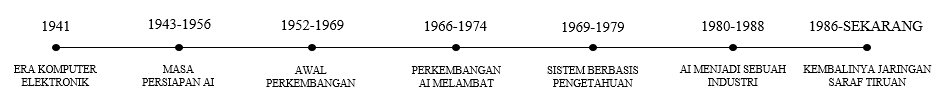
\includegraphics[scale=0.5]{figures/Screenshot_1.png}
\caption{capturing}
\label{perkembangan}
\end{figure}


Ditemukannya pertama kali alat penyimpanan dan pemrosesan informasi yang disebut komputer elektronik. Tahun 1943, Warren McCulloch dan Walter Pitts berhasil membuat suatu model saraf tiruan di mana setiap neuron digambarkan sebagai ‘on’ dan ‘off’. Pada tahun 1950, Norbert Wiener membuat penelitian mengenai prinsip-prinsip teori feedback. Pada tahun 1956, John McCarthy meyakinkan Minsky, Claude Shannon, dan Nathaniel Rochester untuk membantunya melakukan penelitian dalam bidang automata, jaringan saraf, dan pembelajaran intelijensia. Mereka mengerjakan proyek ini selama 2 bulan di Universitas Dartmouth. Hasilnya adalah program yang mampu berpikir non-numerik dan menyelesaikan masalah pemikiran, yang dinamakan Principia Mathematica. Hal ini menjadikan McCarthy disebut sebagai father of Artificial Intelligence/ Bapak Kecerdasan Buatan.

Pada tahun 1958, McCarthy di MIT AI Lab mendefinisikan bahasa pemrograman tingkat tinggi yaitu LISP, yang sekarang mendominasi pembuatan program-program AI. Kemudian, McCarthy membuat program yang dinamakan programs with common sense. Pada tahun 1959, Program komputer General Problem Solver berhasil dibuat oleh Herbert A. Simon, J.C. Shaw, dan Allen Newell. Program ini dirancang untuk memulai penyelesaian masalah secara manusiawi. Pada tahun yg sama Nathaniel Rochester dari IBM dan para mahasiswanya merilis program AI yaitu geometry theorem prover. Pada tahun 1963, program yang dibuat James Slagle mampu menyelesaikan masalah integral tertutup untuk mata kuliah Kalkulus. Pada tahun 1968, program analogi buatan Tom Evan menyelesaikan masalah analogi geometri yang ada pada tes IQ.

Perkembangan AI melambat disebabkan adanya beberapa kesulitan yang di hadapi seperti  Program-program AI yang bermunculan hanya mengandung sedikit atau bahkan tidak mengandung sama sekali pengetahuan pada subjeknya, banyak terjadi kegagalan pada pembuatan program AI, terdapat beberapa batasan pada struktur dasar yang digunakan untuk menghasilkan perilaku intelijensia. Pada tahun 1960an, Ed Feigenbaum, Bruce Buchanan, dan Joshua Lederberg merintis proyek DENDRAL yaitu program untuk memecahkan masalah struktur molekul dari informasi yang didapatkan dari spectometer massa. Pada tahun 1986, program ini telah berhasil menghemat 40 juta dolar per tahun. Pada tahun 1988, kelompok AI di DEC menjalankan 40 sistem pakar. Hampir semua perusahaan besar di USA mempunyai divisi Ai sendiri yang menggunakan ataupun mempelajari sistem pakar. Perusahaan yang sejak tahun 1982 hanya menghasilkan beberapa juta US dollar per tahun meningkat menjadi 2 milyar US dollar per tahun pada tahun 1988.

Meskipun bidang ilmu komputer menolak jaringan saraf tiruan setelah diterbitkannya buku ‘Perceptrons’ karangan Minsky dan Papert, tetapi para ilmuwan masih mempelajari bidang ilmu tersebut dari sudut pandang yang lain, yaitu fisika. Ahli fisika seperti Hopfield (1982) menggunakan teknik-teknik mekanika statistika untuk menganalisa sifat-sifat penyimpanan dan optimasi pada jaringan saraf. Para ahli psikolog, David Rumhelhart dan Geoff Hinton melanjutkan penelitian mengenai model jaringan saraf pada memori. Pada tahun 1985-an sedikitnya empat kelompok riset menemukan algoritma Back-Propagation. Algoritma ini berhasil diimplementasikan ke dalam ilmu bidang komputer dan psikologi.


\item Definisi Supervised Learning
Supervised learning adalah sebuah pendekatan dimana sudah terdapat data yang dilatih, dan terdapat variable yang ditargetkan sehingga tujuan dari pendekatan ini adalah mengkelompokan suatu data ke data yang sudah ada.


\item Klasifikasi dan Regresi
Dalam klasifikasi, keluaran dari setiap data adalah bilangan bulat atau diskrit. Misalnya pengambilan keputusan untuk main sepak bola atau tidak maka keluaran bisa diubah kedalam bilangan bulat 1 (main bola), dan -1 (tidak main). Regresi, keluaran dari setiap data dalah bilangan kontinu. Misalnya peramalan harga rumah berdasarkan lokasi, umur rumah dan luas rumah, maka keluarannya berupa bilangan kontinu berupa bilangan Rp 120 juta, Rp 100 juta atau Rp 51 juta.


\begin{figure}[ht]
\centering
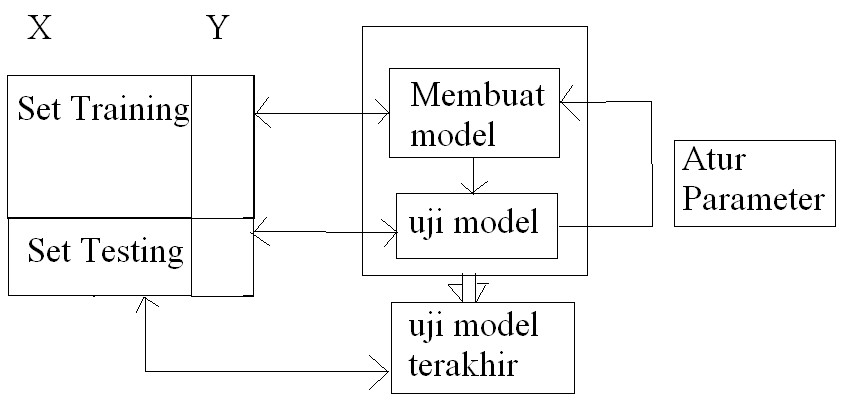
\includegraphics[scale=0.5]{figures/Screenshot_2.jpg}
\caption{capturing}
\label{item}
\end{figure}
\end{enumerate}

\section{Instalasi}
Untuk Instalasinya mencakup i beberapa pembahasan dan tutorial. yaitu :
\begin{enumerate}
\item Instalasi Scikit-Learn Dari Anaconda
\begin{itemize}

\begin{figure}[ht]
\centering
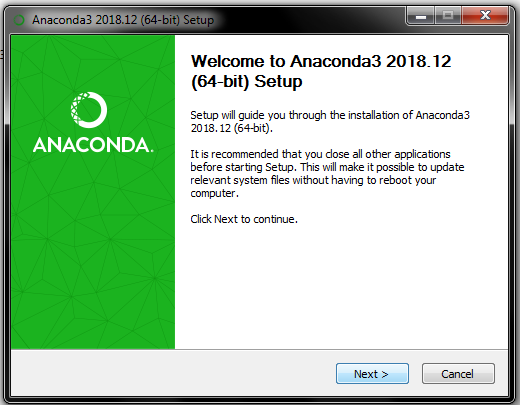
\includegraphics[scale=0.5]{figures/1.png}
\caption{capturing}
\label{proses instalasi}
\end{figure}

\begin{figure}[ht]
\centering
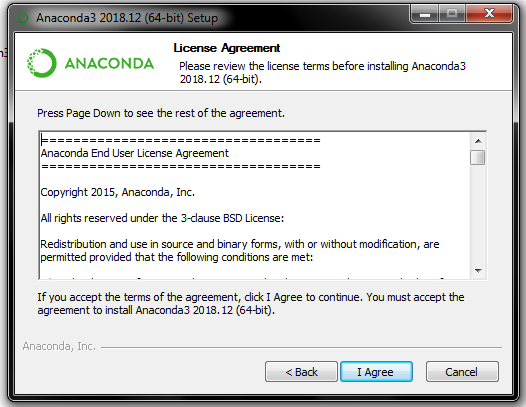
\includegraphics[scale=0.5]{figures/2.png}
\caption{capturing}
\label{proses instalasi}
\end{figure}

\begin{figure}[ht]
\centering
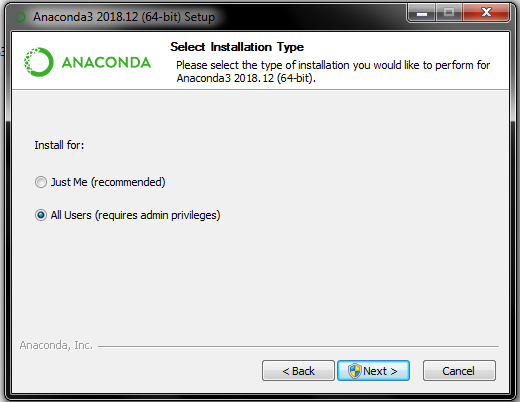
\includegraphics[scale=0.5]{figures/3.png}
\caption{capturing}
\label{proses instalasi}
\end{figure}

\begin{figure}[ht]
\centering
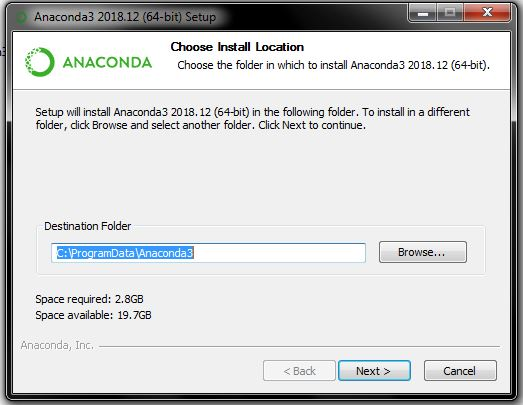
\includegraphics[scale=0.5]{figures/4.jpg}
\caption{capturing}
\label{proses instalasi}
\end{figure}

\begin{figure}[ht]
\centering
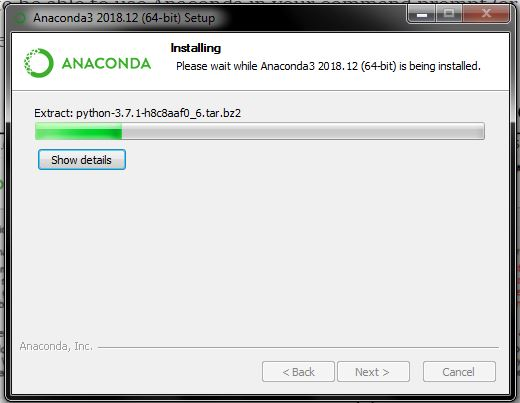
\includegraphics[scale=0.5]{figures/6.jpg}
\caption{capturing}
\label{proses instalasi}
\end{figure}

\begin{figure}[ht]
\centering
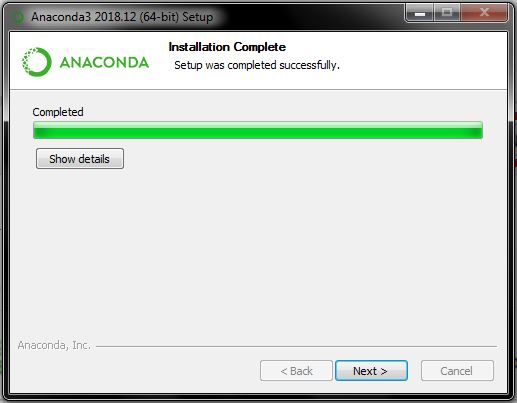
\includegraphics[scale=0.5]{figures/7.jpg}
\caption{capturing}
\label{proses instalasi}
\end{figure}

\begin{figure}[ht]
\centering
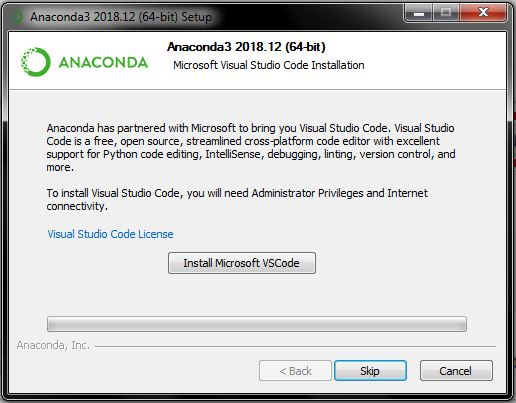
\includegraphics[scale=0.5]{figures/8.jpg}
\caption{capturing}
\label{proses instalasi}
\end{figure}

\begin{figure}[ht]
\centering
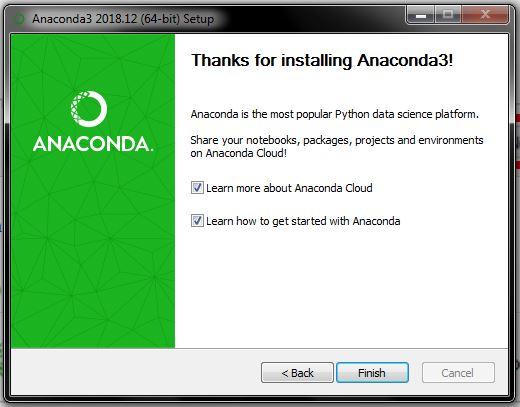
\includegraphics[scale=0.5]{figures/9.jpg}
\caption{capturing}
\label{proses instalasi}
\end{figure}

\begin{figure}[ht]
\centering
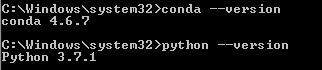
\includegraphics[scale=0.5]{figures/10.jpg}
\caption{capturing}
\label{proses instalasi}
\end{figure}

\begin{figure}[ht]
\centering
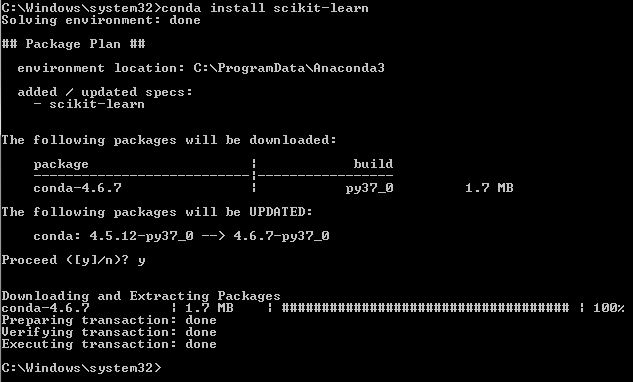
\includegraphics[scale=0.5]{figures/11.jpg}
\caption{capturing}
\label{proses instalasi}
\end{figure}

\begin{figure}[ht]
\centering
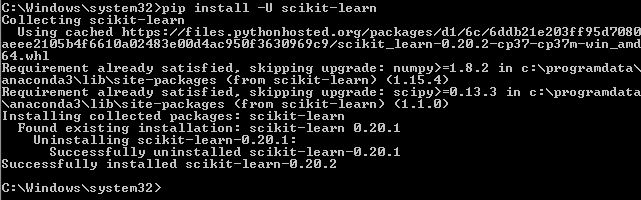
\includegraphics[scale=0.5]{figures/12.jpg}
\caption{capturing}
\label{proses instalasi}
\end{figure}

\begin{itemize}

\item Setelah proses download selesai, run package yang telah didownload lalu next.
\item Pilih 'I Agree' untuk menyetujui persyaratan dan peraturan mengenai aplikasi ini.
\item Lalu, pilih 'All Users' untuk dapat diakses oleh semua user, dan pilih "Just Me' hanya untuk dapat diakses oleh 1 user pc.
\item Kemudian, pilih penyimpanan package.
\item Ceklis pada bagian cek box pertama untuk otomatis pengaturan dan penambahan enviroment variabel pada PATH dan cek box kedua untuk register anaconda sistem.
\item Proses instalasi
\item Lalu pada proses ini, skip untuk mempercepat proses penginstalan.
\item Proses instalasi selesai.
\item Setelah proses instalasi selesai, cek penginstalan conda dan python.
\item Lalu install scikit dengan perintah 'pip install -U scikit-learn" atau 'conda install scikit-learn'
\end{itemize}

\item Instalasi Scikit-Learn Dari Anaconda
\begin{figure}[ht]
\centering
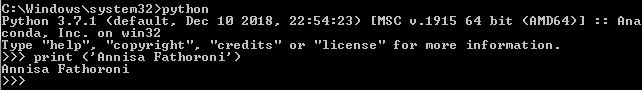
\includegraphics[scale=0.5]{figures/Capture2.jpg}
\caption{capturing}
\label{uji coba}
\end{figure}

Pada uji coba tersebut terdapat variabel 'Annisa Fathoroni' dan jika diprint akan keluar variabel tersebut.
Ini menunjukkan bahwa python telah terhubung dengan anaconda.

\item Mencoba Loading an Example Dataset dan Penjelasan Per-baris

\begin{figure}[ht]
\centering
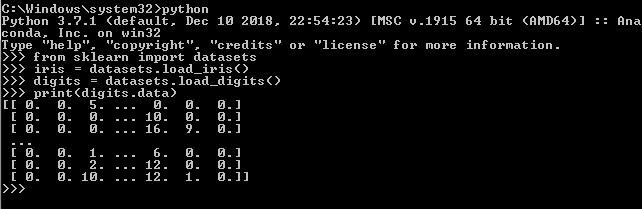
\includegraphics[scale=0.5]{figures/Capture.jpg}
\caption{capturing}
\label{loading an example dataset}
\end{figure}

\item Baris 1:
Memanggil data dari sklearn.
\item Baris 2:
Terdapat variabel 'iris', dimana variabel iris memanggil datasets dan di dalamnya akan memproses digits.
\item Baris 3:
Kemudian ada variabel lainnya 'digits' yang digunakan untuk memanggil dataset dan di dalamnya akan memproses digits.
\item Kemudian untuk perintah Print( digits.data ) untuk menampilkan output dari hasil variabel digits dan akan berupa data.

\end{enumerate} 